\begin{Figure}

    \HEADING{MOOSE makes multiscale modeling easier}

    \TEXT{Rdesigneur (\textbf{R}eaction-\textbf{D}iffusion and
        \textbf{E}lectrical \textbf{SIG}naling in \textbf{NEUR}ons) class makes it
        easier to mix models across scales:}
        
    \TEXT{Following databases/models are supported}
    \begin{itemize}
        \item \TEXT{Neuron morphology and network, \texttt{NeuroMorpho (SWC),
                    NeuroML}}
        \item \TEXT{Chemical pathways, Reaction diffusion models, \texttt{System
                Biology Markup Language (SBML), DOQCS, KKIT}}
        \item \TEXT{Ion-channels models \texttt{channelpedia, OpenSourceBrain}}
    \end{itemize}
    
    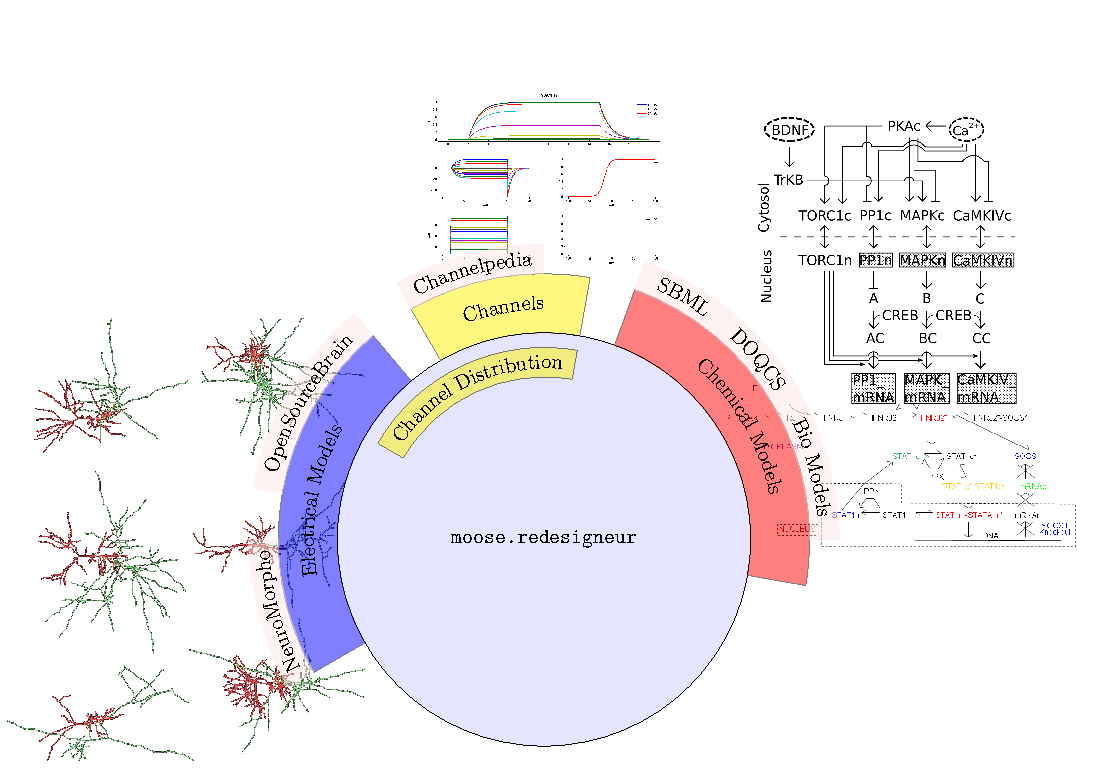
\includegraphics[width=\textwidth]{./_images/rdesigneur.pdf}

    \HEADING{Supported Platforms}

    \TEXT{Packages are available for all major Linux flavors}
    { 
        \includegraphics[width=\textwidth]{./_images/supported_platforms.png}
        \includegraphics[width=\textwidth]{./_images/supported_platforms1.png}
    }

    \HEADING{Summary}
    \begin{itemize}

        \item \TEXT{Designed to be multiscale from the onset. Integrate many
                scales of neuronal data with basic physical/chemical
                principles.}

        \item \TEXT{Rdesigneur makes it easy to mix chemical, electrical and
                channel models in \MOOSE}

        \item \TEXT{Easily scriptable via Python. GUI/3D visualization support}
        \item \TEXT{Packages are available for Linux/MaxOSX. Python-scripting
                interface builds on Windows under Cygwin}

    \end{itemize}

    \TEXT{Source code {\bf https://github.com/BhallaLab/moose}. Packages and
        documentation {\bf http://moose.ncbs.res.in}}

\end{Figure}



